\subsubsection{Generator UUID}
Struktura:
\begin{itemize}
	\item storage/src/shared/storage\_uuid\_srv.erl – gen\_server
\end{itemize}

Jest to wielowątkowy moduł służący do generowania unikalnych, 128-bitowych identyfikatorów. Identyfikatory te są wykorzystywane jako nazwy fizycznych plików przechowywanych w systemie dyskowym. Właściwymi identyfikatorami plików i użytkowników w systemie pozostają jednak zwykłe napisy, w postaci czytelnej dla człowieka.

Strukturę modułu przedstawia diagram z \autoref{fig:uuid-module}. Jedyna publiczna funkcja służy do generowania identyfikatora. Dla każdego wywołania uruchamiany jest osobny wątek. Identyfikator zwracany jest w postaci typu binary().

\begin{figure}[!htbp]
	\centering
	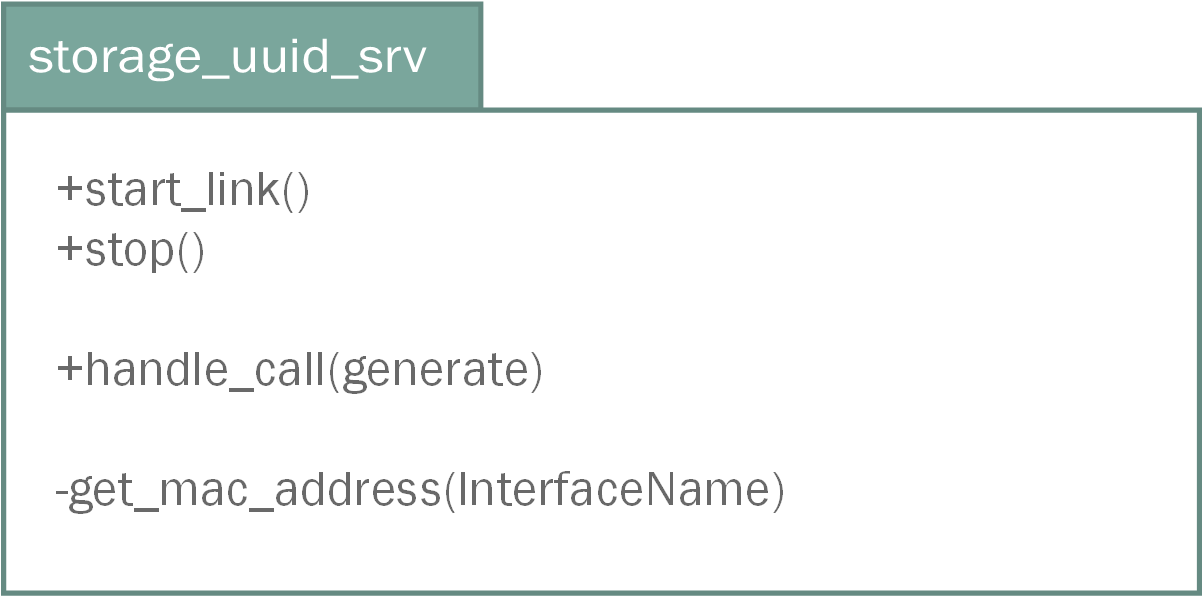
\includegraphics[width=0.7\textwidth]{uuid-module}
	\caption{Interfejs modułu storage\_uuid\_srv.}
	\label{fig:uuid-module}
\end{figure}

Identyfikator składa się z trzech części – grup bitów, z których każda ma odpowiednią interpretację:

\centerline{\texttt{<< 48bit timestamp, 48bit adres MAC, 32bit losowa wartość >>}}

48-bitowy znacznik czasowy przechowuje czas wygenerowania identyfikatora (UNIX time) z dokładnością do milisekund. Adres MAC pobierany jest z określonego w pliku konfiguracyjnym interfejsu sieciowego (domyślnie eth0). Zastosowanie składnika w postaci MAC gwarantuje, że generowane identyfikatory są unikalne w obrębie całego systemu. Ostatni składnik identyfikatora to 32 losowe bity. Daje to 4 294 967 296 możliwych do wygenerowania unikalnych identyfikatorów w ciągu milisekundy.